\appendix
\renewcommand\thechapter{\Alph{chapter}}

\chapter{Lemma on Bounded Solutions}
\label{appendix:lemma-on-bounded-solutions}

\begin{lemma*}[On bounded solutions]
	Let $f(t, z)$ be a function that is continuous with respect to $t$ and continuously differentiable with respect to $z$.
	Let $f(t, z)$ is defined for $t \ge t_0$, $|z| < +\infty$, and have the following properties:
	\begin{itemize}
		\item[(i)] for $|z| < \rho$, $\rho > 0$, the estimate $|f(t, z)| < \eta_{\rho}(t)|z|$ is valid, where $\eta_{\rho}(t) \in L_1(t_0; +\infty)$;
		\item[(ii)] for all $z_1$, $z_2$ such that $|z_{1,2}| < \rho$, $\rho > 0$, there exists function $\tilde{\eta}_{\rho}(t) \in L_1(t_0; +\infty)$, such that $|f(t, z_2) - f(t, z_1)| \le \tilde{\eta}_{\rho}(t) |z_2 - z_1|$;
		\item[(iii)] for $|z| < \rho$, $\rho > 0$, the estimate $|f_z(t, z)| < \theta_{\rho}(t) |z|$ is valid, where $\theta_{\rho} \in L_1(t_0, +\infty)$;
		\item[(iv)] for all $z_1$, $z_2$ such that $z_{1,2} < \rho$, $\rho > 0$, there exists function $\tilde{\theta}_{\rho} \in L_1(t_0; +\infty)$, such that $|f_z(t, z_2) - f_z(t, z_1)| \le \tilde{\theta}_{\rho} |z_2 - z_1|$.
	\end{itemize}
	Then for the equation
	\begin{equation}
		z_{tt} - \alpha z_t + f(t, z) = 0, \quad \alpha > 0
		\label{eq:lemma-bs-main}
	\end{equation}
	the following statements are valid:
	\begin{itemize}
		\item[(A)] for each solution $z(t)$ of the equation \eqref{eq:lemma-bs-main} that is bounded when $t \to +\infty$ there exists $C \in \mathbb{R}$ such that $z(t) \to C$ as $t \to +\infty$;
		\item[(B)] for each $C \in \mathbb{R}$ there exists unique solution $Z(t, C)$ of the equation \eqref{eq:lemma-bs-main}, defined on a segment $(t_C; +\infty)$, such that
		\begin{equation}
			Z(t, C) = C + o(1), \quad t \to +\infty;
		\end{equation}
		\item[(C)] family of solutions $Z(t, C)$ is $C^1$-smooth with respect to the parameter $C$.
	\end{itemize}
\end{lemma*}
\begin{proof}
	Let us prove the statement (A) first.
	With the method of variation of parameters one can find that a solution of the equation \eqref{eq:lemma-bs-main} satisfies the equality:
	\begin{equation}
		z(t) = \varkappa_1 + \varkappa_2 e^{\alpha t} + \int \limits_{t_0}^{t} e^{\alpha \eta} \left( \int \limits_{\eta}^{+\infty} e^{-\alpha \xi} f(\xi, z(\xi)) d\xi \right) d\eta.
	\end{equation}
	It follows from the condition (i) that if $z(t)$ is bounded while $t \to +\infty$ then the integral
	\begin{equation}
		\int \limits_{t_0}^{+\infty} e^{\alpha \eta} \left( \int \limits_{\eta}^{+\infty} e^{-\alpha \xi} f(\xi, z(\xi)) d\xi \right) d\eta
	\end{equation}
	converges.
	Furthermore for all bounded solutions $\varkappa_2 = 0$, hence $z(t)$ tends to some constant for $t \to +\infty$.
	That proves the point (A).
	
	Move on to the point (B).
	We make a variable change $u(t) = z(t) - C$, where $C$ is an arbitrary number.
	Rewrite the equation \eqref{eq:lemma-bs-main} in the form of a system of equations
	\begin{equation}
		y_t = Ay + F(t, y),
		\label{eq:lemma-bs-system}	
	\end{equation}
	where
	\begin{equation*}
		y = \begin{pmatrix}
			u \\ v
		\end{pmatrix}, \quad
		A = \begin{pmatrix}
			0 & 1 \\
			0 & \alpha
		\end{pmatrix}, \quad
		F(t, y) = \begin{pmatrix}
			0 \\ f(t, u + C)
		\end{pmatrix}.
	\end{equation*}
	Now we apply Theorem 9.1 from \cite[Chapter XII]{Hartman} to the system \eqref{eq:lemma-bs-system}.
	It states that the system \eqref{eq:lemma-bs-system} {\it has a solution which tends to zero at infinity} \underline{if} the following conditions are satisfied:
	\begin{itemize}
		\item[(1)] function $F(t, y)$ is continuous and $||F(t, y)|| \le \lambda(t)$ for $t \in [t_0; +\infty)$, $||y|| \le \rho$, where $\lambda(t) \in L_1(t_0; +\infty)$;
		\item[(2)] for all $g(t) = col(g_1(t), g_2(t))$, $g(t) \in L_1(t_0; +\infty)$ there exists a solution $y(t) \in L_0^{\infty}(t_0; +\infty)$ of the inhomogeneous system
		\begin{equation}
			y_t = Ay + g(t);
			\label{eq:lemma-bs-hartman}
		\end{equation}
		(hereinafter by the norm $||\cdot||$ we mean the Euclidean norm in $\mathbb{R}$).
	\end{itemize}
	
	At first, by the condition (i) if $|u| \le \rho$ and $t > t_0$ relation $||f(t, u, C)|| \le \rho \eta_{\rho} (t)$ takes place, moreover $\eta_{\rho} \in L_1(t_0; +\infty)$, hence the condition (1) of the above-mentioned theorem is satisfied.
	At second, general solution of the inhomogeneous system of equations \eqref{eq:lemma-bs-hartman} can be written as:
	\begin{eqnarray}
		&& u(t) = C_2 + \int \limits_{t_0}^{t} \left( g_1(\eta) + e^{\alpha \eta} \left( C_1 - \int \limits_{+\infty}^{\eta} e^{-\alpha \xi} g_2(\xi) d\xi \right) \right) d\eta; \\
		&& v(t) = u_t(t) - g_1(t).
	\end{eqnarray}
	Since $g_{1,2}(t) \in L_1(t_0; +\infty)$ one can choose appropriate parameters $C_1$, $C_2$ in order to get a solution which tends to zero while $t \to +\infty$, so the condition (2) of the theorem is also met.
	Thereby both of the conditions for the applied theorem take place for the system \eqref{eq:lemma-bs-system}.
	That implies existence of a solution $z(t)$ of \eqref{eq:lemma-bs-main} that approaches a given constant $C$ while $t \to +\infty$ for all $C$.
	
	Now we prove the uniqueness of such solution.
	Suppose that for the same $C$ there exist two solutions $u_{1,2}(t)$ for equation
	\begin{equation}
		u_{tt} - \alpha u_t + f(t, u + C) = 0.
		\label{eq:lemma-bs-u}
	\end{equation}
	Consider their difference $\Delta(t) = u_2(t) - u_1(t)$, it satisfies the equation
	\begin{equation}
		\Delta_{tt} - \alpha \Delta_t + R(t) \Delta = 0,
		\label{eq:lemma-bs-difference}
	\end{equation}
	and a boundary condition $\Delta \to 0$ as $t \to +\infty$ takes place.
	Here
	\begin{equation}
		R(t) \equiv \dfrac{f(t, u_2(t) +C) - f(t, u_1(t) + C}{u_2(t) - u_1(t)}.
	\end{equation}
	By the condition (ii) we can apply Theorem 11 from \cite[Chapter 3]{Coppel}.
	It states that there exists a homeomorphism between the bounded solutions of the equation \eqref{eq:lemma-bs-difference} and solutions of equation
	\begin{equation}
		\Delta_{tt} - \alpha \Delta_t = 0,
	\end{equation}
	moreover (see a note to that theorem in \cite{Coppel}) this homeomorphism is a linear map.
	It means that only a zero solution of \eqref{eq:lemma-bs-difference} satisfies the zero asymptotic at infinity, i.e. $u_2(t) \equiv u_1(t)$.
	Thus we have proven the existence of the solutions family $Z(t, C)$ parametrised by $C \in \mathbb{R}$, statement (B) is proven.
	
	To prove the statement (C) one can note that the derivative
	\begin{equation}
		\dfrac{\partial Z}{\partial C}(t, C) \equiv \Theta(t, C)
	\end{equation}
	satisfies the equation \eqref{eq:lemma-bs-u} after differentiation with respect to $C$, moreover $\Theta(t, C) \to 0$ as $t \to +\infty$.
	We have
	\begin{equation}
		\Theta_{tt} - \alpha \Theta_t + f_z(t, u + C) \Theta + f_z(t, u + C) = 0.
	\end{equation}
	Here we can use Theorem 11 from \cite[Chapter 3]{Coppel} again, and using the condition (iii) we can conclude that there exists a solution of this equation $\Theta(t, C)$ such that $\Theta(t, C) \to 0$ as $t \to +\infty$, and function $\Theta(t, C)$ is continuous with respect to the parameter $C$.
	That proves the overall lemma.
\end{proof}

\chapter{Solutions of Duffing equations}
\label{appendix:solutions-of-duffing-equations}

\chapter{Strips Mapping Theorems}
\label{appendix:strips-mapping-theorems}

% TODO: Where is Conley-Moser conditions? Cite Wiggins somewhere.
% TODO: Read through this carefully.
\begin{theorem}[On h-strips mapping]
	Let Poincar\'e map $\mathcal{P}$ and its inverse $\mathcal{P}^{-1}$ are defined on a complete (see Definition~\ref{def:complete-island-set}) island set $\bigcup_{i \in S} D_i$, where $S$ is a finite or countable set of indices.
	Let for all $i, j \in S$ set $V_{ji} = \mathcal{P}^{-1} D_j \cap D_i$ is non-empty, $\mathcal{P}$ is defined on a
	 closure $\overline{V_{ji}}$, and one of the following two conditions is met:
	\begin{enumerate}
		\item[(1)] borders $\alpha_i^{\pm}$ of an island $D_i$ are increasing curves, $\forall \vb{p} \in \overline{V_{ji}}$ signs of values $\{ a_{mn} \}$ in the matrix of the linear operator $D \mathcal{P}_{\vb{p}} = (a_{mn})$ have exactly one of the following configurations\footnote{By ``$+$'' and ``$-$'' sign we mean \underline{strict} inequalities $a_{mn} > 0$, $a_{mn} < 0$ to be held.}:
			\begin{center}
				(a) $\begin{psm} + & + \\ + & + \end{psm}$, \quad
				(b) $\begin{psm} - & - \\ - & - \end{psm}$, \quad
				(c) $\begin{psm} + & + \\ - & - \end{psm}$, \quad
				(d) $\begin{psm} - & - \\ + & + \end{psm}$;
			\end{center}
			and at the same time borders $\alpha_j^{\pm}$ of $D_j$ are increasing curves for cases (a), (b), and decreasing curves for (c), (d);
		\item[(2)] borders $\alpha_i^{\pm}$ of an island $D_i$ are decreasing curves, $\forall \vb{p} \in \overline{V_{ji}}$ signs of values $\{ a_{mn} \}$ in the matrix of the linear operator $D \mathcal{P}_{\vb{p}} = (a_{mn})$ have exactly one of the following configurations:
			\begin{center}
				(a) $\begin{psm} + & - \\ - & + \end{psm}$, \quad
				(b) $\begin{psm} - & + \\ + & - \end{psm}$,	\quad
				(c) $\begin{psm} + & - \\ + & - \end{psm}$, \quad
				(d) $\begin{psm} - & + \\ - & + \end{psm}$;		
			\end{center}
			and at the same time borders $\alpha_j^{\pm}$ of $D_j$ are decreasing curves for cases (a), (b), and increasing for (c), (d);
	\end{enumerate}
	and moreover $\exists \mu > 1$ such that $\forall p \in \overline{V_{ji}}$, $|a_{11}| \ge \mu$, then for any \emph{h}-strip $H \in D_i$, $\mathcal{P} (H) \cap D_j = \widetilde{H}_j$ is also an \emph{h}-strip, and $d_{\mathrm{h}}(\widetilde{H}_j) \le (1 / \mu) d_{\mathrm{h}}(H)$ (here $d_{\mathrm{h}}(\cdot)$ is an \emph{h}-strip thickness in a sence of Definition~\ref{def:h-thickness}).
\end{theorem}
\begin{proof}
	Let's fix indices $i, j$ and prove the theorem for a pair of islands $D_i$, $D_j$.
	Mostly we consider the case (1а).
	Other cases 
	The rest of the cases must be treated in a completely analogous way.
	Denote by $\mathbf{e}_1$, $\mathbf{e}_2$ basis vectors
	\begin{equation}
		\mathbf{e}_1 = \begin{pmatrix} 1 \\ 0 \end{pmatrix}; \quad \mathbf{e}_2 = \begin{pmatrix} 0 \\ 1 \end{pmatrix}.
	\end{equation}
	Define the following set of {\it cones}:
	\begin{align*}
		\mathbb{R}_{++}^2 = \{ \mathbf{v} \, | \, \mathbf{v} = x \mathbf{e}_1 + y \mathbf{e}_2, \; x > 0, y > 0 \}; \\
		\overline{\mathbb{R}}_{++}^2 = \{ \mathbf{v} \, | \, \mathbf{v} = x \mathbf{e}_1 + y \mathbf{e}_2, \; x \ge 0, y \ge 0 \}; \\
		\mathbb{R}_{+-}^2 = \{ \mathbf{v} \, | \, \mathbf{v} = x \mathbf{e}_1 + y \mathbf{e}_2, \; x > 0, y < 0 \}; \\
		\overline{\mathbb{R}}_{+-}^2 = \{ \mathbf{v} \, | \, \mathbf{v} = x \mathbf{e}_1 + y \mathbf{e}_2, \; x \ge 0, y \le 0 \}; \\
		\mathbb{R}_{-+}^2 = \{ \mathbf{v} \, | \, \mathbf{v} = x \mathbf{e}_1 + y \mathbf{e}_2, \; x < 0, y > 0 \}; \\
		\overline{\mathbb{R}}_{-+}^2 = \{ \mathbf{v} \, | \, \mathbf{v} = x \mathbf{e}_1 + y \mathbf{e}_2, \; x \le 0, y \ge 0 \}; \\
		\mathbb{R}_{--}^2 = \{ \mathbf{v} \, | \, \mathbf{v} = x \mathbf{e}_1 + y \mathbf{e}_2, \; x < 0, y < 0 \}; \\
		\overline{\mathbb{R}}_{--}^2 = \{ \mathbf{v} \, | \, \mathbf{v} = x \mathbf{e}_1 + y \mathbf{e}_2, \; x \le 0, y \le 0 \}. \\
	\end{align*}
	As a \underline{first} step in the proof, we show that values signs in the matrix of linear operator $D \mathcal{P}_{\vb{p}} = ( a_{mn} )$ uniquely determine the structure of cones mapping in each point $\vb{p}$ of the set $\overline{V_{ji}}$.
	For the case (a) we have:
	\begin{equation*}
	\forall \mathbf{v} = \begin{pmatrix} x \\ y \end{pmatrix} \in \overline{\mathbb{R}}_{++}^2, \ D \mathcal{P}_{\vb{p}}(\mathbf{v}) = \begin{pmatrix} a_{11} & a_{12} \\ a_{21} & a_{22} \end{pmatrix} \begin{pmatrix} x \\ y \end{pmatrix} = \begin{pmatrix} \widetilde{x} > 0 \\ \widetilde{y} > 0\end{pmatrix} \in \mathbb{R}_{++}^2.	
	\end{equation*}
	It is easy to check that the complete scheme of the cones mapping for the case (1) of the theorem looks as follows:
	\begin{eqnarray*}
		(\textup{a}) & D \mathcal{P}_{\vb{p}} (\overline{\mathbb{R}}_{++}^2) \in \mathbb{R}_{++}^2, \quad D \mathcal{P}_{\vb{p}} (\overline{\mathbb{R}}_{--}^2) \in \mathbb{R}_{--}^2; \\
		(\textup{b}) & D \mathcal{P}_{\vb{p}} (\overline{\mathbb{R}}_{++}^2) \in \mathbb{R}_{--}^2, \quad D \mathcal{P}_{\vb{p}} (\overline{\mathbb{R}}_{--}^2) \in \mathbb{R}_{++}^2; \\
		(\textup{c}) & D \mathcal{P}_{\vb{p}} (\overline{\mathbb{R}}_{++}^2) \in \mathbb{R}_{+-}^2, \quad D \mathcal{P}_{\vb{p}} (\overline{\mathbb{R}}_{--}^2) \in \mathbb{R}_{-+}^2; \\
		(\textup{d}) & D \mathcal{P}_{\vb{p}} (\overline{\mathbb{R}}_{++}^2) \in \mathbb{R}_{-+}^2, \quad D \mathcal{P}_{\vb{p}} (\overline{\mathbb{R}}_{--}^2) \in \mathbb{R}_{+-}^2.
	\end{eqnarray*}
	Complete scheme for the case (2) have the following form correspondingly:
	\begin{eqnarray*}
		(\textup{a}) & D \mathcal{P}_{\vb{p}} (\overline{\mathbb{R}}_{-+}^2) \in \mathbb{R}_{-+}^2, \quad D \mathcal{P}_{\vb{p}} (\overline{\mathbb{R}}_{+-}^2) \in \mathbb{R}_{+-}^2; \\
		(\textup{b}) & D \mathcal{P}_{\vb{p}} (\overline{\mathbb{R}}_{-+}^2) \in \mathbb{R}_{+-}^2, \quad D \mathcal{P}_{\vb{p}} (\overline{\mathbb{R}}_{+-}^2) \in \mathbb{R}_{-+}^2; \\
		(\textup{c}) & D \mathcal{P}_{\vb{p}} (\overline{\mathbb{R}}_{-+}^2) \in \mathbb{R}_{--}^2, \quad D \mathcal{P}_{\vb{p}} (\overline{\mathbb{R}}_{+-}^2) \in \mathbb{R}_{++}^2; \\
		(\textup{d}) & D \mathcal{P}_{\vb{p}} (\overline{\mathbb{R}}_{-+}^2) \in \mathbb{R}_{++}^2, \quad D \mathcal{P}_{\vb{p}} (\overline{\mathbb{R}}_{+-}^2) \in \mathbb{R}_{--}^2.
	\end{eqnarray*}
	
	As a \underline{second} step we show that such cones mapping preserve in some way Lipschitz constraints and monotonicity properties for curves from $\overline{V_{ji}}$ under the $\mathcal{P}$ mapping.
	Show that for the case (1a).
	For that first of all we note that from compactness of $\overline{V_{ji}}$ the existence of the following supremum follows:
	\begin{equation*}
		\widetilde{\gamma}_{ji} = \sup \dfrac{y}{x}, \ \begin{pmatrix} x \\ y \end{pmatrix} = D \mathcal{P}_{\vb{p}} (\mathbf{v}), \ \vb{p} \in \overline{V_{ji}}, \ \mathbf{v} \in \overline{\mathbb{R}}_{++}^2.
	\end{equation*}
	Further, let there be two tow different points $\vb{p}_1 \, \vb{p}_2 \in \overline{V_{ji}}$, $\vb{p}_1 = (\psi_1, \psi_1')$, $\vb{p}_2 = (\psi_2, \psi_2')$, and besides $\psi_2 \ge \psi_1$, $\psi_2' \ge \psi_2$.
	Let points $\vb{q}_1$, $\vb{q}_2$ be the $\mathcal{P}$-images of the points $\vb{p}_1$, $\vb{p}_2$ correspondingly, $\mathcal{P}(\vb{p}_1) = \vb{q}_1 = (\phi_1, \phi_1')$, $\mathcal{P}(\vb{p}_2) = \vb{q}_2 = (\phi_2, \phi_2')$.
	Let $D \mathcal{P}_{\vb{p}_1}$ is a linearization of $\mathcal{P}$ at the point $\vb{p}_1$.
	Then the following expansion is valid:
	\begin{equation}
		\vb{q}_2 = \mathcal{P}(\vb{p}_2) = \vb{q}_1 + D \mathcal{P}_{\vb{p}_1} (\vb{p}_2 - \vb{p}_1) + r(||\vb{p}_2 - \vb{p}_1||),
	\end{equation}
	where $r(||\vb{p}_2 - \vb{p}_1||) / ||\vb{p}_2 - \vb{p}_1|| \to 0$ as $||\vb{p}_2 - \vb{p}_1|| \to 0$ (here $|||\cdot||$ is a Euclidean norm).
	Vector $\vb{p}_{\Delta} = \vb{p}_2 - \vb{p}_1 \in \overline{\mathbb{R}}_{++}^2$ which means that for its mapping by linearized operator we have $D \mathcal{P}_{\vb{p}_1} (\mathbf{p}_{\Delta}) = \mathbf{q}_{\Delta} \in \mathbb{R}_{++}^2$, and
	\begin{equation}
		\vb{q}_2 - \vb{q}_1 = \mathbf{q}_{\Delta} + r(||\vb{p}_2 - \vb{p}_1||).
	\end{equation}
	Expression above means that for ``close enough'' points $\vb{p}_1$, $\vb{p}_2$ their images satisfy the relationship $\vb{q}_2 - \vb{q}_1 \in \mathbb{R}_{++}^2$, i.e. $\phi_2 > \phi_1$, $\phi_2' > \phi_1'$.
	Moreover one can choose a value $\gamma_{ji} > \widetilde{\gamma_{ji}}$ such that the following inequality is held:
	\begin{equation}
		0 < \phi_2' - \phi_1' < \gamma_{ji} (\phi_2 - \phi_1).
	\label{eq:ordering}
	\end{equation}
	This ordering is transitive, i.e. from the relation \eqref{eq:ordering} and the second analogous relation for ``close enough'' point $\vb{p}_2$, $\vb{p}_3$,
	\begin{equation}
		0 < \phi_3' - \phi_2' < \gamma_{ji} (\phi_3 - \phi_2),
	\end{equation}
	follow the analogous relation for the points $\vb{p}_1$, $\vb{p}_3$ as well.
	That allows to spread the relation \eqref{eq:ordering} over all points $\vb{p}_1, \, \vb{p}_2 \in \overline{V_{ji}}$ that satisfies the conditions $\psi_2 \ge \psi_1$, $\psi_2' \ge \psi_1'$.
	Other cases (1b)-(1d), (2a)-(2d) can be considered in a similar way.
	
	Thus for the case (1) for all points $\vb{p}_1, \, \vb{p}_2 \in \overline{V_{ji}}$, which coordinates satisfy the relations $\psi_2 \ge \psi_1$, $\psi_2' \ge \psi_1'$, coordinates of their $\mathcal{P}$-images $\vb{q}_1 = (\phi_1, \phi_1'), \, \vb{q}_2~=~(\phi_2, \phi_2')$ depending on sings of values in matrix of $D \mathcal{P}_{\vb{p}}$, $\vb{p} \in \overline{V_{ji}}$, met exactly one of the following inequalities ($\exists \gamma_{ji}$):
	\begin{subequations}
	\begin{eqnarray}
		(\textup{a}) & 0 < \phi_2' - \phi_1' < \gamma_{ji} (\phi_2 - \phi_1); \label{eq:ordering_1a} \\
		(\textup{b}) & 0 < \phi_1' - \phi_2' < \gamma_{ji} (\phi_1 - \phi_2); \label{eq:ordering_1b} \\
		(\textup{c}) & 0 < \phi_1' - \phi_2' < \gamma_{ji} (\phi_2 - \phi_1); \label{eq:ordering_1c} \\
		(\textup{d}) & 0 < \phi_2' - \phi_1' < \gamma_{ji} (\phi_1 - \phi_2). \label{eq:ordering_1d}
	\end{eqnarray}
	\end{subequations}
	For the case (2) in its turn we have that for all points $\vb{p}_1, \, \vb{p}_2 \in \overline{V_{ji}}$, which coordinates satisfy the relations $\psi_2 \le \psi_1$, $\psi_2' \ge \psi_1'$, exactly one of the following inequalities is met:
	\begin{subequations}
	\begin{eqnarray}
		(\textup{a}) & 0 < \phi_2' - \phi_1' < \gamma_{ji} (\phi_1 - \phi_2); \label{eq:ordering_2a} \\
		(\textup{b}) & 0 < \phi_1' - \phi_2' < \gamma_{ji} (\phi_2 - \phi_1); \label{eq:ordering_2b} \\
		(\textup{c}) & 0 < \phi_1' - \phi_2' < \gamma_{ji} (\phi_1 - \phi_2); \label{eq:ordering_2c} \\
		(\textup{d}) & 0 < \phi_2' - \phi_1' < \gamma_{ji} (\phi_2 - \phi_1). \label{eq:ordering_2d}
	\end{eqnarray}
	\end{subequations}
	
	A a \underline{third} step we demonstrate how these inequalities above allow to conclude that for any h-strip $H \in D_i$ its image $\mathcal{P} H \cap D_j = \widetilde{H}_j$ is also an h-strip.
	Let an h-strip $H \in D_i$ is placed between two monotonic h-curves $\widetilde{\alpha}_i^{\pm}$.
	Endpoints of the $\widetilde{\alpha}_i^{\pm}$ belong to the boundaries $\beta_i^{\pm}$ of island $D_i$, so the $H$ is a curvilinear quadrangle bounded by curves $\widetilde{\alpha}_i^{\pm}$ and segments of curves $\beta_i^{\pm}$.
	For the case (1a) of the theorem curves $\widetilde{\alpha}_i^{\pm}$  are increasing.
	Let's consider an image of the curve $\widetilde{\alpha}_i^+$.
	According to the definition of a complete island set $\mathcal{P} (\widetilde{\alpha}_i^+)$ cross each of the boundaries $\beta_j^{\pm}$ of island $D_j$ at least once.
	At the same time $\mathcal{P} (\widetilde{\alpha}_i^+)$ cannot cross boundaries $\alpha_j^{\pm}$ because they consist of points which tends to infinity under action of $\mathcal{P}^{-1}$.
	
	Let $\mathcal{P} (\widetilde{\alpha}_i^+)$ cross one of the boundaries $\beta_j^{\pm}$ of the island $D_j$ twice.
	Denote those intersection points by $\vb{q}_1 = \mathcal{P}(\vb{p}_1), \, \vb{q}_2 = \mathcal{P}(\vb{p}_2)$.
	For the case (1a) boundaries $\alpha_j^{\pm}$ are increasing curves, and $\beta_j^{\pm}$ are decreasing, hence the points $\vb{q}_1, \, \vb{q}_2$ belong to a decreasing curve.
	From the other side points $\vb{p}_1, \, \vb{p}_2 \in \overline{V_{ji}}$ belong to increasing curve $\widetilde{\alpha}_i^+$, and hence for their $\mathcal{P}$-image coordinates $\vb{q}_1 = (\phi_1, \phi_1'), \, \vb{q}_2 = (\phi_2, \phi_2')$ inequality \eqref{eq:ordering_1a} must be held.
	This inequality means that points $\vb{q}_1, \, \vb{q}_2$ cannot belong to a decreasing curve, and $\mathcal{P} (\widetilde{\alpha}_i^+)$ cross each boundary $\beta_j^{\pm}$ only once.
	Similar statement is valid also for the $\mathcal{P} (\widetilde{\alpha}_i^-)$.
	% TODO: Add a remark on Lipschitz conditions here.
	Thereby $\mathcal{P} (\widetilde{\alpha}_i^{\pm}) \cap D_j$ are monotonic curves.
	Their type of monotonicity coincide with the monotonicity type of corresponding boundaries of the island $D_j$, moreover these curves bound the set $\mathcal{P} H \cap D_j$, hence $\mathcal{P} H \cap D_j = \widetilde{H}_j$ is an h-strip.
	Other cases can be considered in a similar way using the corresponding inequalities \eqref{eq:ordering_1b} -- \eqref{eq:ordering_1d}, \eqref{eq:ordering_2a} -- \eqref{eq:ordering_2d}.
	
	Finally, in a \underline{fourth} step of this proof we show that under the introduced constrain on $|a_{11}|$ value of linearized operator, for all h-strip $H \in D_i$, $\rho (\widetilde{H}_j) \le \mu \rho(H)$, so that thickness of an h-strip $\mathcal{P}$-image within island $D_j$ is less than thickness of an original h-strip inside island $D_i$.
	To prove that first assume that h-strips $H$ and $\widetilde{H}_j$ are well-measured in a sense on Definition~\ref{def:well-measurable-h-strip}.
	Let the thickness of the h-strip $\widetilde{H}_j$ can be measured along the vertical curve connecting points $\vb{q}_1 = (\phi_1, \phi_1'), \, \vb{q}_2 = (\phi_2, \phi_2')$, $\phi_1' < \phi_2'$.
	Consider a parametrization of that curve $\vb{q}(t) = (0, \phi'(t))$, where
	\begin{equation}
		\phi'(t) = t \phi_2' + (1 - t) \phi_1', \quad 0 \le t \le 1.
	\end{equation}
	Strip $\widetilde{H}_j$ is well-measurable, so the curve $\vb{q}(t)$ entirely belongs to $\widetilde{H}_j$.
	Since $\widetilde{H}_j = \mathcal{P} H \cap D_j$ there exists a pre-image $\vb{p}(t) = \mathcal{P}^{-1} (\vb{q}(t)) = (\psi(t), \psi'(t))$, $\vb{p}(t) \subset H$ and $\vb{q}(t) = \mathcal{P} (\vb{p}(t))$.
	For the case (1a) let's demonstrate that $\vb{p}(t)$ is a decreasing curve connecting point from the opposite boundaries $\widetilde{\alpha}_i^{\pm}$ of the strip $H$ inside $D_i$.
	Remark, here by ``decreasing'' we mean that the curve is a graph of decreasing function in $(u, u')$ coordinates, not as a function of $t$.
	The curve $\vb{q}(t)$ belongs to some set which is a $\mathcal{P}$-image of a part of the set $\overline{V_{ji}}$.
	The signs of values in the matrix of $D \mathcal{P}_{\vb{p}}$, $\vb{p} \in \overline{V_{ji}}$ have the form $\begin{psm} + & + \\ + & + \end{psm}$, so the signs of values for the linearized inverse map $D \mathcal{P}^{-1}_{\vb{q}}$ have a configuration $\begin{psm} + & - \\ - & + \end{psm}$ on the curve $\vb{q}(t)$.
	This allows to conclude the corresponding cones mapping:
	\begin{equation}
		D \mathcal{P}^{-1}_{\vb{q}(t)} (\overline{\mathbb{R}}_{-+}^2) \in \mathbb{R}_{-+}^2, \quad D \mathcal{P}^{-1}_{\vb{q}(t)} (\overline{\mathbb{R}}_{+-}^2) \in \mathbb{R}_{+-}^2.
	\label{eq:cones-backward}
	\end{equation}
	Therefore the corresponding monotonicity property \eqref{eq:ordering_2a} takes place.
	It immediately follows from \eqref{eq:ordering_2a} that the vertical curve $\vb{q}(t)$ is mapped to the decreasing curve $\vb{p}(t)$ (decreasing in $(u, u')$ coordinates).
	Moreover the inequality $\phi_1' < \phi_2'$ provides that $\psi'(t) > 0$.
	
	% TODO: Consider to color left strip as well (for all three pictures).
	\begin{figure}[h]
	\centering
		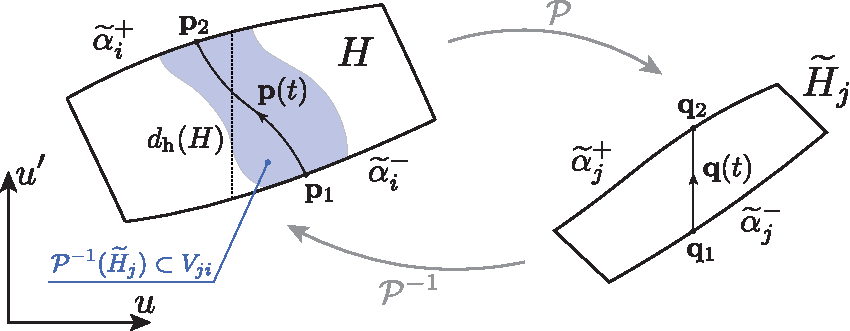
\includegraphics[scale = 1]{pic/thickness of h-strip (a)}
		\caption{
			Illustration for the proof of the h-strips thickness decrease for the case when both h-strips $H$ and $\widetilde{H}_j$ and well-measurable.
			Thickness of $H$ is measured along the vertical dotted line, thickness of $\widetilde{H}_j$ is measured along the vertical line $\vb{q}(t)$.
			Arrows indicate curves traverse directions while $t$ changes from $0$ to $1$.
			Pre-image of $\widetilde{H}_j$ strip is colored with gray.
		}
	\label{fig:thickness-of-h-strip-a}
	\end{figure}
	
	Consider tangent vectors to $\vb{p}(t)$ and $\vb{q}(t)$ (upper dot means the derivative with respect to $t$):
	\begin{eqnarray}
		&& \dot{\vb{p}}(t) = (\dot{\psi}(t), \dot{\psi}'(t)); \\
		&& \dot{\vb{q}}(t) = (0, \dot{\phi}'(t)).
	\end{eqnarray}
	In each point $t$ they are connected by the $D \mathcal{P}_{\vb{p}(t)}$ operator
	\begin{equation}
		\dot{\vb{q}}(t) = D \mathcal{P}_{\vb{p}(t)} (\dot{\vb{p}}(t)).
	\end{equation}
	Rewrite this relation in a matrix form:
	\begin{equation}
		\begin{pmatrix}
			a_{11}(t) & a_{12}(t) \\ a_{21}(t) & a_{22}(t)
		\end{pmatrix}
		\begin{pmatrix}
			\dot{\psi}(t) \\
			\dot{\psi}'(t)
		\end{pmatrix} =
		\begin{pmatrix}
			0 \\ \dot{\phi}'(t)
		\end{pmatrix}.
	\end{equation}
	% TODO: Give a cite, from where follows this fact for Poincar\'e map.
	We take into account that matrix $(a_{mn})$ is a linearization of Poincar\'e map to conclude that its determinant $a_{11}(t) a_{22}(t) - a_{12}(t) a_{21}(t) = 1$ in each point $t$.
	From the relations above and the theorem condition on values of $a_{11}(t)$ follows
	\begin{equation}
		\dot{\phi}'(t) = \dfrac{1}{a_{11}(t)} \dot{\psi}'(t) \le \dfrac{1}{\mu} \dot{\psi}'(t).
	\label{eq:to-integrate}
	\end{equation}
	Integration of \eqref{eq:to-integrate} with limits $0 \le t \le 1$ gives:
	\begin{equation}
		d_{\mathrm{h}}(\widetilde{H}_j) = \phi_2' - \phi_1' = \int \limits_0^1 \dot{\phi}'(t) dt \le \dfrac{1}{\mu} \int \limits_0^1 \dot{\psi}'(t) dt = \dfrac{1}{\mu} (\psi_2' - \psi_1').
	\label{eq:thickness-of-strip-final}
	\end{equation}
	Curve $\vb{p}(t)$ is decreasing and boundaries of $H$ are increasing curves, so it follows from general geometric considerations that $\psi_2' - \psi_1' \le d_{\mathrm{h}}(H)$, i.e. $d_{\mathrm{h}}(\widetilde{H}_j) \le (1 / \mu) d_{\mathrm{h}}(H)$.
	That gives the final statement of the theorem for well-measurable strips.
	
	\begin{figure}[h]
	\centering
		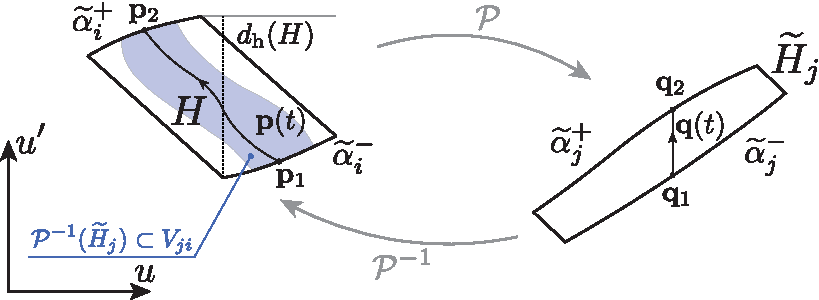
\includegraphics[scale = 1]{pic/thickness of h-strip (b)}
		\caption{
			Illustration for the proof of the h-strips thickness decrease for the case when strip $H$ is not well-measurable.
			Its thickness is measured along the vertical dotted line.
			One endpoint of that line does not belong to the strip boundary $\widetilde{\alpha}_i^+$.
			Pre-image of $\widetilde{H}_j$ strip is colored with gray.
		}
	\label{fig:thickness-of-h-strip-b}
	\end{figure}
	
	The proof above can be easily generalized to the cases when h-strips  $H$ and $\widetilde{H}_j$ are not well-measurable.
	If strip $H$ is not well-measurable, the inequality $\psi_2' - \psi_1' \le d_{\mathrm{h}}(H)$ in \eqref{eq:thickness-of-strip-final} takes place anyway.
	This fact is illustrated on Figure~\ref{fig:thickness-of-h-strip-b}.
	Vertical distance between points $\vb{p}_1, \, \vb{p}_2$ turns out to be certainly less than the width of $H$ strip.
	
	In the case when h-strip $\widetilde{H}_j$ is not well-measurable, one should choose corner points $\vb{q}_1, \, \vb{q}_2$ in a such way that the vertical distance between them equals the thickness of $\widetilde{H}_j$, and then connect $\vb{q}_1, \, \vb{q}_2$ with a monotonic decreasing curve $\vb{q}(t)$, see Fig.~\ref{fig:thickness-of-h-strip-c}.
	This is always possible due to the geometric properties of not well-measurable h-strip.
	According to the choice of points $\vb{q}_1, \, \vb{q}_2$, $d_{\mathrm{h}}(\widetilde{H}_j) = \phi_2 - \phi_1$, and all the steps above remain valid since the corresponding cones mapping with all the consequences can be also applied for the decreasing curves $\vb{p}(t)$ and $\vb{q}(t)$.
	\begin{figure}[h]
	\centering
		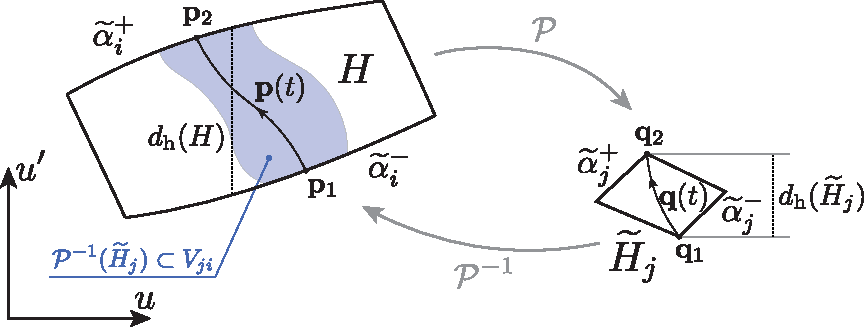
\includegraphics[scale = 1]{pic/thickness of h-strip (c)}
		\caption{
			Illustration for the proof of the h-strips thickness decrease for the case when strip $\widetilde{H}_j$ is not well-measurable.
			Thickness of $H$ and $\widetilde{H}_j$ are measured along the dotted lines.
			Pre-image of $\widetilde{H}_j$ strip is colored with gray.
	  }
	\label{fig:thickness-of-h-strip-c}
	\end{figure}
	
	If both h-strips $H$ and $\widetilde{H}_j$ are not well-measurable then two above mentioned technics should be combined together.
	During the consideration of all other cases of the theorem only type of curves monotonicity is changed, but the overall approach remains the same and can be applied with just minor adjustments.
	Theorem is proven.
\end{proof}

\pagebreak

\begin{theorem}[On v-strips mapping]
	Let Poincar\'e map $\mathcal{P}$ and its inverse $\mathcal{P}^{-1}$ are defined on a complete (see Definition~\ref{def:complete-island-set}) island set $\bigcup_{i \in S} D_i$, where $S$ is a finite or countable set of indices.
	Let for all $i, j \in S$ set $H_{ij} = \mathcal{P} D_i \cap D_j$ is non-empty, $\mathcal{P}^{-1}$ is defined on a
	 closure $\overline{H_{ij}}$, and one of the following two conditions is met:
	\begin{enumerate}
		\item[(1)] borders $\beta_j^{\pm}$ of an island $D_j$ are increasing curves, $\forall \vb{q} \in \overline{H_{ij}}$ signs of values $\{ b_{mn} \}$ in the matrix of the linear operator $D \mathcal{P}_{\vb{q}}^{-1} = (b_{mn})$ have exactly one of the following configurations:
			\begin{center}
				(a) $\begin{psm} + & + \\ + & + \end{psm}$, \quad
				(b) $\begin{psm} - & - \\ - & - \end{psm}$, \quad
				(c) $\begin{psm} + & + \\ - & - \end{psm}$, \quad
				(d) $\begin{psm} - & - \\ + & + \end{psm}$;
			\end{center}
			and at the same time borders $\beta_i^{\pm}$ of $D_i$ are increasing curves for cases (a), (b), and decreasing curves for (c), (d);
		\item[(2)] borders $\beta_j^{\pm}$ of an island $D_j$ are decreasing curves, $\forall \vb{q} \in \overline{H_{ij}}$ signs of values $\{ b_{mn} \}$ in the matrix of the linear operator $D \mathcal{P}_{\vb{q}}^{-1} = (b_{mn})$ have exactly one of the following configurations:
			\begin{center}
				(a) $\begin{psm} + & - \\ - & + \end{psm}$, \quad
				(b) $\begin{psm} - & + \\ + & - \end{psm}$,	\quad
				(c) $\begin{psm} + & - \\ + & - \end{psm}$, \quad
				(d) $\begin{psm} - & + \\ - & + \end{psm}$;		
			\end{center}
			and at the same time borders $\beta_i^{\pm}$ of $D_i$ are decreasing curves for cases (a), (b), and increasing for (c), (d);
	\end{enumerate}
	and moreover $\exists \nu > 1$ such that $\forall q \in \overline{H_{ij}}$, $|b_{22}| \ge \nu$, then for any \emph{v}-strip $V \in D_j$, $\mathcal{P}^{-1} (V) \cap D_i = \widetilde{V}_i$ is also a \emph{v}-strip, and $d_{\mathrm{v}} (\widetilde{V}_i) \le (1 / \nu) d_{\mathrm{v}} (V)$ (here $d_{\mathrm{v}}(\cdot)$ is an \emph{v}-strip thickness in a sence of Definition~\ref{def:v-thickness}).
\end{theorem}
\begin{proof}
	Completely analogous to the proof of the h-strips mapping theorem.
\end{proof}